

\subsection{CAN Controller Software}
\catalin{Explain the code in more detail. Also mention the interrupt part for gpio.}
\catalin{Bullet list: What other functionalities? And, 1st letters capitals or not?}
\catalin{Better titles}
\martin{Write introduction explaining that this code is for testing, because we were missing the link betwen linux and CAN.}
\subsubsection{Main Functionalities}~\\
As mentioned in section \ref{sub:Basic_SourceCode}, the code was based on the xcanps polled example available by Xilinx documentation.
The important functionalities that needed to be provided by the final software version included:
\begin{itemize}
\item receiving and sending of frames
\item creating the message id
\item decoding of the message id parts, such as the node id, the message type and the command
\item handling interrupts from buttons and a GPIO port
\item controlling the LEDs
\martin{buttons and leds aren't part of the final software? Or are we still talking about the software for testing?}
\item accepting and ignoring messages according to a subscriptions list
\end{itemize}

\subsubsection{Publisher-Subscriber Architecture}
\catalin{Should I explain more about the architecture? Or is it the readers responsibility to read about it?}
A mechanism was also necessary to control the receivers and transmitters of messages.
One of the functionalities of the network was to provide the ability for various nodes to be able to send specific messages to other nodes.
Such a mechanism could easily be implemented using the Publisher-Subscriber architecture which would also make the network data-driven.
Using this method, the communication among the various nodes could be easily configured just by adding messages ids to an array variable containing the node's subscriptions.
The use of this architecture was incorporated in the protocol functionality, along with a set of functions in the source code and an array variable of subscriptions for each node.

\subsubsection{Main Loop}
Since the whole system, that was intended to be designed for this project, could not be put together, an approach to simulate the network in various ways was needed.
Specifically, sending arbitrary messages was achieved by implementing button interrupts
%\martin{I removed some text, that doesn't fit with the validation part}
%and the case where multiple nodes would send messages simultaneously by GPIO port interrupts.
%For details on how the different tests were done the reader may refer to section \ref{sub:CAN_Bus_Tests}.
%Due to conflicts between the interrupt controllers and handlers, only one of the two simulation cases could be active during runtime.
%Depending on the value of a macro definition in the source code the desired devices (buttons or GPIO) would be initialized.

\paragraph{Button Interrupts Runtime}~\\
As seen in behavioral diagram in figure \ref{fig:StateDiagram_CANSoft_BtnsIntr}, the program waits for button pushes or for receiving data in the FIFO in the main loop.
In the former case, a message is sent to the network containing the value of the pushed buttons, while in the latter case, the data is decoded and the appropriate value is written to the LEDs as output.
\begin{figure}[h!]
	\centering
	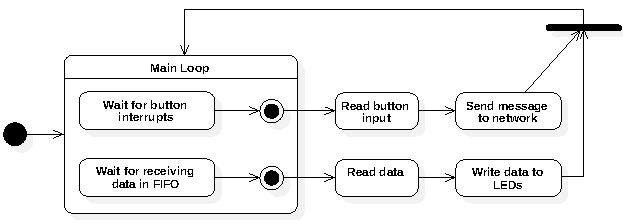
\includegraphics[width = 1\linewidth]{graphics/StateDiagram_CANSoft_BtnsIntr.pdf}
	\caption{Behavioral diagram with button interrupts.}
	\label{fig:StateDiagram_CANSoft_BtnsIntr}
\end{figure}

\paragraph{GPIO Interrupts Runtime}~\\
\martin{Do we use this? I didn't use interrupts for my code}
The software's behavior is similar in this case, as well as it can be seen in figure \ref{fig:StateDiagram_CANSoft_GPIOIntr}.
The difference is that instead of button values, dummy data may be inserted into the TxFrame according to the simulation needs and the receiving data is only presented in the SDK terminal.
\begin{figure}[h!]
	\centering
	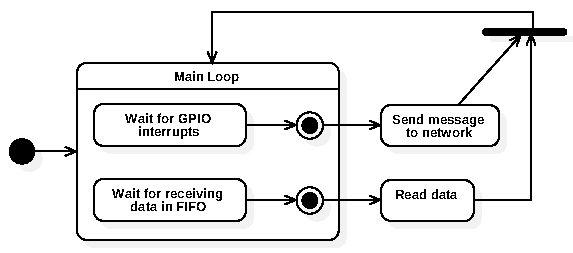
\includegraphics[width = 0.85\linewidth]{graphics/StateDiagram_CANSoft_GPIOIntr.pdf}
	\caption{Behavioral diagram with GPIO interrupts.}
	\label{fig:StateDiagram_CANSoft_GPIOIntr}
\end{figure}

\subsubsection{Sending and Receiving Frames}
\martin{We probably should document something about the xcanps examples used in the verification}
\martin{Describe createMsgID()?}
The figure \ref{fig:SeqDiagram_SendFrame} shows the procedure of sending a frame to the CAN network containing data, which makes use of the protocol function createMsgID().
After returning the message id, the id and the data are put into the TxFrame to be sent once the FIFO has space.
The actual sending is done with a call to the XCanPs function XCanPs\_Send().
\\
Similarly, the procedure of receiving a frame is shown in the figure \ref{fig:SeqDiagram_RecvFrame}.
The node once it calls the RecvFrame() function, it waits in a loop until it receives a frame.
Then, it checks the subscriptions in order to forward the packet for further processing or to ignore it.
In both cases appropriate messages using the function xil\_printf() are presented to the developer in the SDK terminal.

\begin{figure}[h!]
	\centering
	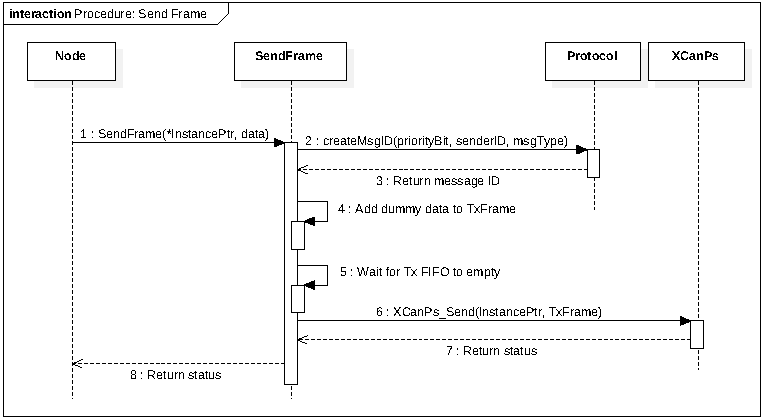
\includegraphics[width = 1\linewidth]{graphics/SeqDiagram_SendFrame.pdf}
	\caption{The sequence diagram of the process of sending a frame.}
	\label{fig:SeqDiagram_SendFrame}
\end{figure}

\begin{figure}[h!]
	\centering
	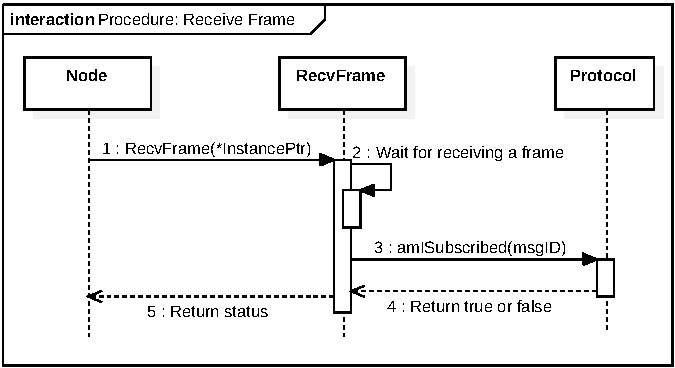
\includegraphics[width = 1\linewidth]{graphics/SeqDiagram_RecvFrame.pdf}
	\caption{The sequence diagram of the process of receiving a frame.}
	\label{fig:SeqDiagram_RecvFrame}
\end{figure}